%%%%%%%%%%%%%%%%%%%%%%%%%%%%%%%%%%%%%%%%%%
%%%%%%%%%%%%%                 %%%%%%%%%%%%
%%%%%%%%%%%%%    EXERCISE 1   %%%%%%%%%%%%
%%%%%%%%%%%%%                 %%%%%%%%%%%%
%%%%%%%%%%%%%%%%%%%%%%%%%%%%%%%%%%%%%%%%%%
\begin{exercise}[]{An adventure game uses a graph $G$ consisting of $N$ rooms (numbered from $1$ to $N$) to represent the places need to be explored. These rooms can only be linked in one-way, meaning that a person passing through this path can only move from one room to another but cannot return to the room they left/explored. It’s worth noting that there is no circle in this graph. People taking part in the game appear randomly in any of the rooms connected via corridors, and we can explore rooms in the same corridor. You should note that the path taken by two players may contain some of the same rooms.

    How many players are the minimum needed to explore all the rooms?
    
    Describe your design first and write down your algorithm in the form of pseudo-code.}
  \begin{solution} If no edges are used, then the number of players required to explore the room is simply $N$. If two rooms are reachable from one to the other, then we can let one player explore them in a single pass. Furthermore, all the rooms on the connected path can also be explored by a single player. Therefore, if we find a connected matching, we can reduce the player required by 1. To minimize the players is equivalent to maximize the matching. Since paths can use the same node, we should first use a Floyd algorithm to get a table of connectivity for matching usage. The matching problem can be solved in a network flow model.

  \begin{algorithm}[h]
    \caption{Explore Room}
    \KwIn{rooms $r_1,\ldots,r_N$, connectivity $(i,j)\in E$}
    \KwOut{$m$ the minimum number of players to explore all the rooms}
    \BlankLine
    Initialize an 2-d array $R[N][N]$ to be all False indicating the connectivity of all nodes\;
    \For{$(i,j)\in E$}{
      $R[i][j] = True$\;
    }
    \For{$i = 1 \ldots N$}{
      \For{$j=1\ldots N$}{
        \For{$k=1\ldots N$}{
          \If{$R[i][k] \& R[k][j] = True$}{
            $R[i][j] = True$\;
          }
        }
      }
    }
    Build a network graph, let $s$ connect $x_1,\ldots,x_N$ nodes and $y_1,\ldots,y_n$ pointed to $t$.\;
    Link $x_i$ and $y_j$ if $R[i][j]$ is true, assign unit capacity to all the edges\;
    Run ford-fulkerson algorithm on the network graph the find the maximum flow $F$\;
    \Return{$N-F$}\;
  \end{algorithm}
  \end{solution}
  \label{ex1}
\end{exercise}


%%%%%%%%%%%%%%%%%%%%%%%%%%%%%%%%%%%%%%%%%%
%%%%%%%%%%%%%                 %%%%%%%%%%%%
%%%%%%%%%%%%%    EXERCISE 2   %%%%%%%%%%%%
%%%%%%%%%%%%%                 %%%%%%%%%%%%
%%%%%%%%%%%%%%%%%%%%%%%%%%%%%%%%%%%%%%%%%%
\begin{exercise}[]{Suppose there are $M \times N$ rooms, each of which holds a different number of treasures. Please select several rooms so that the selected rooms have no common sides (i.e., the selected rooms cannot be adjacent), and the selected rooms' treasures add up to the greatest value.
    Describe your design first and write down your algorithm in the form of pseudo-code.
    
    Note: The value of the treasure is definitely not negative.}
  \begin{solution} The problem can be solved by dynamic programming. We can find the suboptimal structure of the problem by constructing a 2d table $DP$. $DP[i][j]$ indicate the maxmimal value of the treasures in the range from rooms ranging in rows from 1 to i and columns from 1 to j. Then the optimal solution for arbitrary $DP[i][j]$ can be obtained by exploting the solution of its optimal substructure. (Note: in the following algorithm, for simplicity, max() will ignore invalid arguments)

  \begin{algorithm}[H]
    \KwIn{The value of treasure $v[i][j]$ for every room in $M\times N$}
    \KwOut{A set of $(i,j)$ rooms to collect treasure}
    \BlankLine
    Create a table $DP[M][N]$ and initialize to 0\;
    \For{$j=1...N$}{
      $DP[1][j] = \max(DP[i][j-2] + v[1][j], DP[1][j-1])$
    }
    \For{$i=2:M$}{
      \For{$j=1:N$}{
        $DP[i][j] = \max(DP[i][j-2] + v[i][j],DP[i-2][j]+ v[i][j], DP[i-1][j], DP[i][j-1],DP[i-1][j-1]])$
      }
    }
    Initialize solution set $S$ to be empty\;
    Initialize current index $i = M, j = N$\;
    \While{$i>0$ or $j>0$}{
      Check whether $DP[i][j]$ is equal to any of its predecessor neighbors, if yes, modify $i,j$ to that node \;
      Check whether $DP[i][j]-v[i][j]$ is equal to $DP[i][j-2]$ or $DP[i-2][j]$ \;
      If yes, append the current node into $S$ and then modify $i,j$\;
    }
    \Return{S}
    \caption{Treasure Discovering}
  \end{algorithm}


  % dp on a playground
  \end{solution}
  \label{ex2}
\end{exercise}


%%%%%%%%%%%%%%%%%%%%%%%%%%%%%%%%%%%%%%%%%%
%%%%%%%%%%%%%                 %%%%%%%%%%%%
%%%%%%%%%%%%%    EXERCISE 3   %%%%%%%%%%%%
%%%%%%%%%%%%%                 %%%%%%%%%%%%
%%%%%%%%%%%%%%%%%%%%%%%%%%%%%%%%%%%%%%%%%%
\begin{exercise}[]{There are a large number of servers in the data center. Each server has different performance, the program is executed on different servers with different efficiency, and now there is a set of the new programs that need to run. Please assign these programs to the appropriate server based on the historical test results to make this batch of programs run most efficiently. 
    Describe your design first and write down your algorithm in the form of pseudo-code.
    }
  \begin{solution}
  \par{~}
  In this problem, we need to find a maximum matching between servers $S$ and programs $P$, which can be solved using Kuhn and Munkres Algorithm. Note that the server and programs may not match in total number, so we should preprocess them.



  \begin{algorithm}[H]
    \KwIn{The score of performance of program $i$ on server $j$ $v[i][j]$ for $M$ programs and $N$ servers}
    \KwOut{An assignment of $(i,j)$s}
    \BlankLine
    Create a graph with $M$ program and $N$ server nodes. Connect program $i$ to server $j$ with edge value $v[i][j]$ \;
    \If{M<N}{
      Add $N-M$ dummy programs and assign them with 0 value to every server, making $M=N$\;
    }
    \If{N<M}{
      Add $N-M$ dummy servers and assign them with 0 value to every programs, making $N=M$\;
    }
    Assign a feasible $ell$ for $G$, namely, $\ell(v)=0$ for all $v \in P$ and $\ell(u)=\max _{v \in S}\{v(u, v)\}$ for all $u \in P .$\;
    \Return{Kuhn-Munkres(G,$\ell$)}
    \caption{Server Dispatching}
  \end{algorithm}
  % Dummy progs
  % 打分
  % max weight bip-matching

  In this algorithm we will assign a label $\ell(v)$ to all nodes $v \in S \cup P$. We say that a labeling is feasible iff $\ell(u)+\ell(v) \geq v(u, v)$ for all $(u, v) \in P \times S .$  Note that there always exists a feasible labeling of a bipartite graph, namely $\ell(v)=0$ for all $v \in P$ and $\ell(u)=\max _{v \in S}\{v(u, v)\}$ for all $u \in P .$
  
  Next we denote an equality subgraph to be $G_{=}=\left(P, S, E_{=}\right)$. It is identical to $G$ except that $E_{=}=\{(u, v) \in E$ $\ell(u)+\ell(v)=v(u, v)\} .$ 
  
  We have a theorem that, if there exists a perfect matching $M^{*}$ in the equality subgraph $G_{=},$ then $M^{*}$ is an optimal assignment in $G$.

  Now the job left for us is to maintain a equality subgraph that can yield the matching solution. And then run the Hungrarian Algorithm on the subgraph.

  \begin{algorithm}[H]
    \KwIn{Bipartite Graph $G$ and a matching$M$ to be agumented}
    \KwOut{An optimal perfect matching $M$ on $G$, or an evidence $E$ that no perfect matching exists}
    \BlankLine
    \eIf{$M$ is a perfect matching}{
      \Return{M}
    }{
      $u \leftarrow$ a vertex in $P$ unmatched in $M$ \;
      Build an alternating tree $T$ from $u$ \;
      \eIf{an unmatched vertex $v \in S$ is found when building $T$}
      {use the path from $u$ to $v$ to augment $M,$ yielding $M^{\prime}$ \;
      \Return{Hungarian $\left(G, M^{\prime}\right)$}
      }
      {$E \leftarrow T \cap P$\;
        \Return{ $E$ as evidence that no perfect matching exists}
      }

    }
    \caption{Hungarian Algorithm}
  \end{algorithm}

  As Kuhn Munkres proceeds forward, when no more matching can be found in $G_{=}$, we need to modify the label(line 14 - 15). Line 14 finds an edge not yet in $G_{=}$ and then creates a new labeling that will bring that edge into $G_{=}$ on the recursive call. This step will guarantee all edges will be added if necessary and they will be added in the order that decreases the sum of total weight as little as possible at each step. This order, in particular, ensures that our algorithm will yield the optimal solution.

  \begin{algorithm}[H]
    \KwIn{Bipartite Graph $G$ and a feasible $\ell$ value assignment}
    \KwOut{An optimal perfect matching on $G$}
    \BlankLine
    $G_{=} \leftarrow$ the equality subgraph induced by $\ell$\;
    $M \leftarrow$ any matching in $G_{=}$, discovered by Hungarian Algorithm \;
    \eIf{$M$ is a perfect matching}{\label{code}
      \Return{M}
    }{
    let $u \in P$ be an unmatched vertex in $M$\;
    \While{$Neighbor(E)\neq T$, where $S$ is the evidence set returned by Hungarian when the graph has no perfect matching}{
      grow the alternating tree $T$\;
      \If{a new matching $M^{\prime}$ is found}{
        $M \leftarrow M^{\prime}$\;
        goto \ref{code}
      }
    }
    $\alpha_{\ell} \leftarrow \min _{x \in S,  y \notin T}\{\ell(x)+\ell(y)-v(x, y)\}$ \;
    For all $v\in P \cup S$,  $\bar{\ell}(v) \leftarrow\left\{\begin{array}{ll}\ell(v)-\alpha_{\ell} & \text { if } v \in S \\ \ell(v)+\alpha_{\ell} & \text { if } v \in T \\ \ell(v) & \text { otherwise }\end{array}\right.$
    }
    \Return{Kun-Munkres(G,$\ell$)}
    \caption{Kuhn Munkres Max Weight Matching}
  \end{algorithm}

  

  \end{solution}
  \label{ex3}
\end{exercise}


%%%%%%%%%%%%%%%%%%%%%%%%%%%%%%%%%%%%%%%%%%
%%%%%%%%%%%%%                 %%%%%%%%%%%%
%%%%%%%%%%%%%    EXERCISE 4   %%%%%%%%%%%%
%%%%%%%%%%%%%                 %%%%%%%%%%%%
%%%%%%%%%%%%%%%%%%%%%%%%%%%%%%%%%%%%%%%%%%
\begin{exercise}[]{Given a weighted directed graph $G(V, E)$ and its corresponding weight matrix $W=(w_{ij})_{n \times n}$ and shortest path matrix $D=(d_{ij})_{n \times n}$, where $w_{ij}$ is the weight of edge $(v_i, v_j)$ and $d_{ij}$ is the weight of a shortest path from pairwise vertex $v_i$ to $v_j$. Now, assume the weight of a particular edge $(v_a, v_b)$ is decreased from $w_{ab}$ to $w'_{ab}$. Design an algorithm to update matrix $D$ with respect to this change, whose time complexity should be no larger than $O(n^2)$. Describe your design first and write down your algorithm in the form of pseudo-code.}
  \begin{solution}
  \par{~}
  Assume all the weights are nonnegative, since the modification will only affect the paths that pass $(a,b)$, we can for every pair of points $(x,y)$, check if the pass $x\rightarrow a \rightarrow b \rightarrow y$ will cost less than the original $d(x,y)$. This work can be done in a single pass, since $d(x,a)$ and $d(b,y)$ will certainly not be affected by $w(a,b)$. After iterating all pairs, the update is done in $O(n^2)$ time.

  \begin{algorithm}[H]
    \KwIn{weight matrix $W=(w_{ij})_{n \times n}$ and shortest path matrix $D=(d_{ij})_{n \times n}$, $w'_{ab}$}
    \KwOut{shortest path matrix $D=(d_{ij})_{n \times n}$}
    \BlankLine
    \For{x=1...N}{
      \For{y=1...N}{
        \If{$d(x,a)+w'(a,b)+d(b,y) < d(x,y)$}{
          $d(x,y) = d(x,a)+w'(a,b)+d(b,y)$
        }
      }
    }\Return{$D$}
    \caption{Update shortest distance}
  \end{algorithm}
  
  \end{solution}
  \label{ex4}
\end{exercise}


%%%%%%%%%%%%%%%%%%%%%%%%%%%%%%%%%%%%%%%%%%
%%%%%%%%%%%%%                 %%%%%%%%%%%%
%%%%%%%%%%%%%    EXERCISE 5   %%%%%%%%%%%%
%%%%%%%%%%%%%                 %%%%%%%%%%%%
%%%%%%%%%%%%%%%%%%%%%%%%%%%%%%%%%%%%%%%%%%
\begin{exercise}[]{Please review the papers to find an algorithmic problem related to the non-obvious network flow or circulation problem, summarize its problem formulation, and transform it into the network flow problem.
    
    }
  \begin{solution}
  \par{~}
  \paragraph{Background} Compiler Optimization used to take a lot of complexity in computation due to the implicit, complicated data-flow information in the control flow model. However, the emergence of \textbf{SSA-form} (Single Static Assignment) has help resolve this issue by modifying the traditional control flow graph by inserting $\phi$-nodes (which in semantics means that the value of the assigned can be either in the arguments) and renaming variables with an extra index to make sure that every SSA-variable is defined only once, and its definition will always dominate its uses (i.e. all paths from entry to a use will pass through its def).

  % ssa example
  \begin{figure}
    \centering
    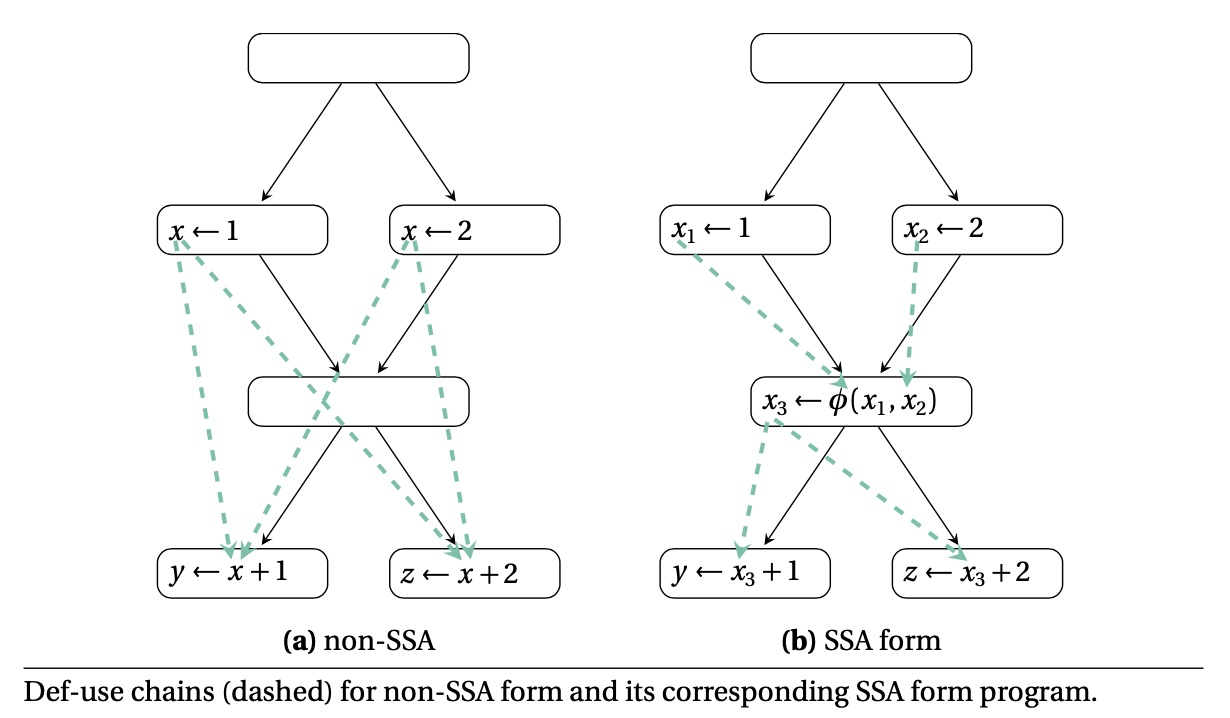
\includegraphics[width=8cm]{img/ex6-ssa.jpg}
    \caption{SSA Example}
    \label{ssa}
  \end{figure}

  The construction of SSA can be done in an iterative way. After such transformation, the dominance property of SSA can help accelarate many traditional optimization algorithms since the life cycle of every variable will be explicitly implied from the SSA version of control flow graph. For example, data flow analysis can be done in a 2-pass traverse and no longer requires iteration to solve the data flow equation. In fact, modern compilers such as LLVM, GCC have been adopting or transforming SSA-methods. Almost all optimizations performed by the Maple Compiler of HUAWEI (also known as FANGZHOU Compiler) are based on SSA-form programs.

  The problem we are focusing on here is called \textbf{partial redundancy elimination}(PRE) problem. In this problem, we should eliminate expressions redudant on \textit{some} (not necessarily all) paths. A case in point can be found in Figure \ref{pre}. Note that not all paths will have the expression $a+b$ as we want to eliminate. However, an additional instruction (called \textit{speculation}) can be added so that $B4,B5$ can reuse the pre-computed results, creating a potential improvement in performance during runtime. The problem is that speculation is not always beneficial. Let's say we have a profile of the program that the frequency of executing the speculated branch is higher, the cost of additional computation will outweigh the return of redundancy elimination.
  
  \begin{figure}
    \centering
    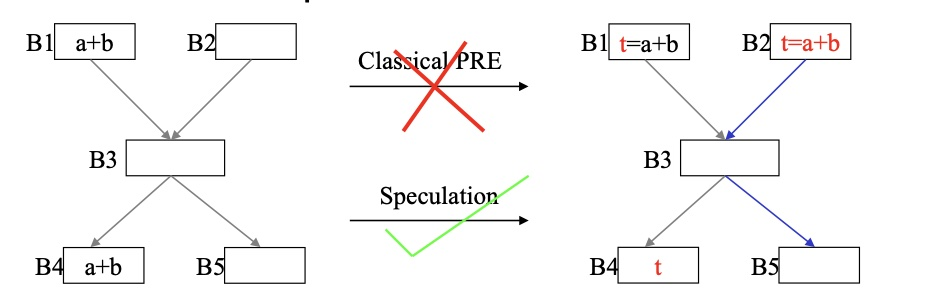
\includegraphics[width=12cm]{img/ex6-pre1.jpg}
    \caption{Partial redundancy elimination Example}
    \label{pre}
  \end{figure}
  \begin{figure}
    \centering
    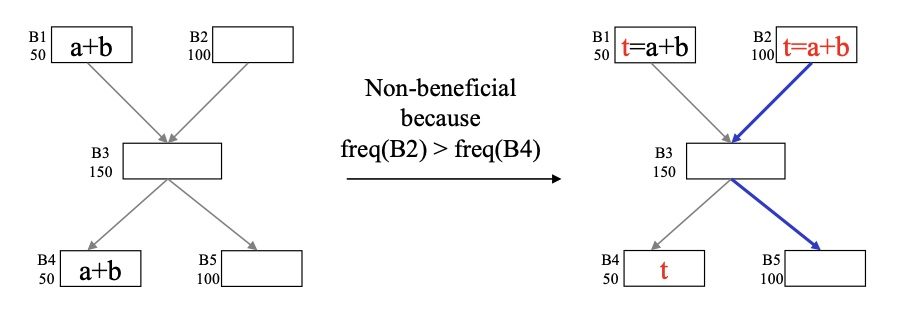
\includegraphics[width=12cm]{img/ex6-pre2.jpg}
    \caption{An example that Partial redundancy elimination doesn't help}
    \label{pre2}
  \end{figure}

  In traditional non-SSA-form, \textit{Cai and Xue} first apply min-cut to propose a computationally and lifetime optimal algorithm for speculative PRE based on profile data. Their algorithm uses bit-vector-based data-flow analysis and applies minimum cut to flow networks formed out of the control-flow graph to find the optimal code placement. \textit{Zhou et al.} applies the minimum cut approach to flow networks formed out of the FRG in the SSAPRE framework to achieve the same computational and lifetime optimal code motion, and furthermore showing that in SSA-form, the optimal code placements can be computed more efficiently. 
  
  Here, we focus on Zhou's PRE algorithm based on SSA-form since it is more efficient and useful given that SSA is receiving growing attention in compiler techniques today.

  \paragraph{Problem Statement}  The key problem in PRE is to decide where and whether to insert speculation given the profile of a problem, in order to minimize the dynamic execution count of an expression. 
  
  In SSA-PRE framework, we can represent expressions in a similar way to SSA-form variables by assigning them to a \textit{hypothetical temporary} $h$, forming a \textbf{factored redundancy graph}(FRG), shown in \ref{frg}. We insert the corresponding $\phi$-nodes to make the FRG have the dominance property. With such representation, the input program is more compact and more efficient to analyze.

  Now we extract three kinds of nodes from the FRG, connected by arrows in Figure\ref{frg}:
  \begin{enumerate}
    \item $h_1$, $h_2$, ... represent real occurences in the original program, which can either be def(always non-redundant) or use(partially redundant, or fully redudant, should be analyzed to eliminate). Of course, those fully redundant nodes can be eliminated during preprocessing (a procedure called \textit{Graph Reduction}), so we won't bother discussing them in later procedures.
    \item $h$ defined by $\phi$
    \item $h$ used in $\phi()$ operands, which can be $\bot$
  \end{enumerate}

  \begin{figure}
    \centering
    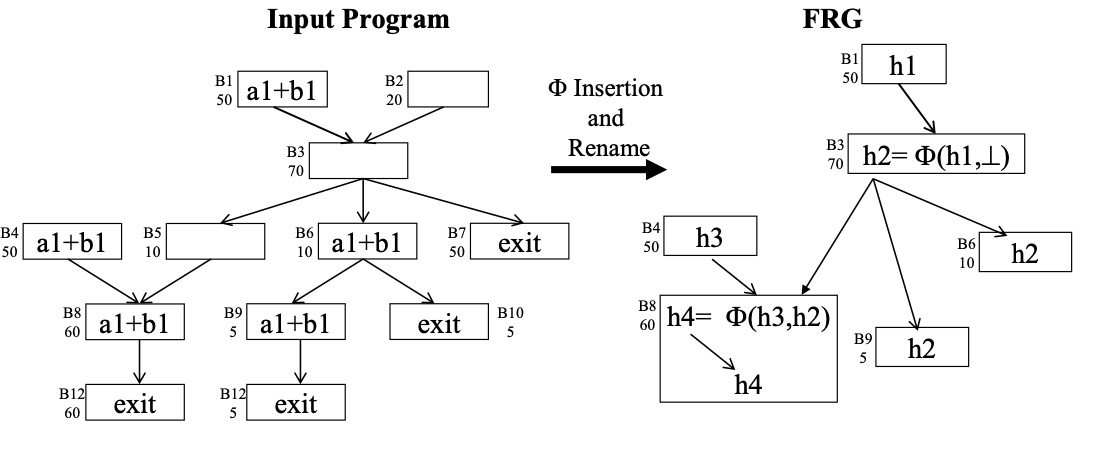
\includegraphics[width=12cm]{img/ex6-frg.jpg}
    \caption{Factored redundancy graph}
    \label{frg}
  \end{figure}

  As has been mentioned above, we only care about those nodes where \textit{partial} redundancy happens, so we can shrink a lot of nodes which are fully available or not partial anticipated at all. A reduced graph for the above FRG is shown in Figure \ref{red}

  \begin{figure}
    \centering
    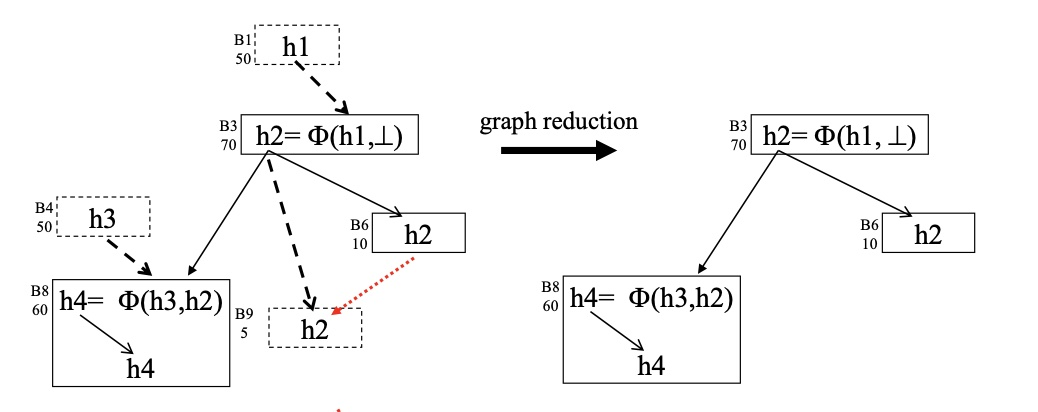
\includegraphics[width=12cm]{img/ex6-red.jpg}
    \caption{Reduced redundancy graph}
    \label{red}
  \end{figure}

  Now the problem is reduced to follows: on the reduced graph, for every $h$ (hypothetical temporary), we should determine whether to add a speculation or not. The author argues that this non-obvious decision problem can be formulated as a min-cut problem that can be solved through classical network flow approaches with modifications as follows.

  \paragraph{Network Formulation}
  \begin{enumerate}
    \item Introduce a virtual source node, add an edge from it to each undefined $\bot$ in $\phi(\ldots,\bot)$ operand.
    \item Introduce a virtual sink node, add an edge from each real occurence to it.
    \item For each edge in the flow network formed above, assign capacity as follows:
    \begin{enumerate}
      \item Edges to the sink are never insertion candidate, so mark them as $\infty$ capacity
      \item For edges ending at a $\phi$ operand, an insertion at such edge indicates inserting at the exit of all its predecessor basic block corresponding to the $\phi$ operand. Thus, we should mark them with the profile frequency of that particular predecessor basic block. They are marked as Type 1 edge in Figure \ref{flow}
      \item For edges from a $\phi$ def to a real occurence, an insertion at such edge indicates performing the computation in place. Thus, we should mark them with the node frequency of the real occurence being pointed. They are marked as Type 2 edge in Figure \ref{flow}
    \end{enumerate}
      \item By performing a minimum cut computation, we can find the optimal insertion points in the cut edge set. In this algorithm, later cuts are picked in case of ties to ensure life-cycle optimality.
      \item Process the program according to the cut edges found and the semantics of the edges indicated above, shown in \ref{restore}.
  \end{enumerate}


  \begin{figure}
    \centering
    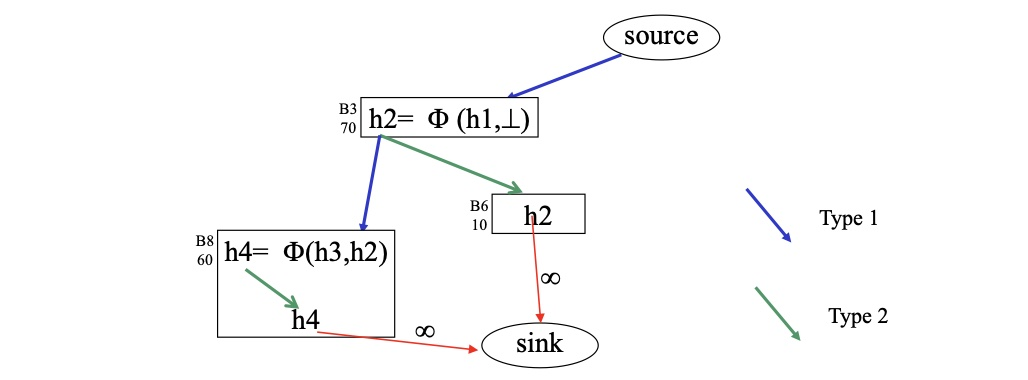
\includegraphics[width=12cm]{img/ex6-flow.jpg}
    \caption{Network Formulation}
    \label{flow}
  \end{figure}

  \begin{figure}
    \centering
    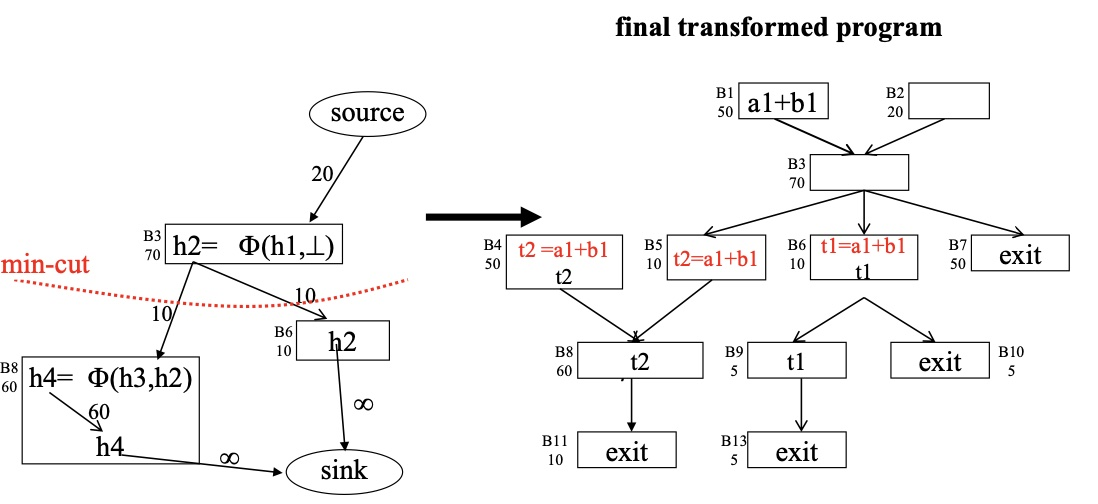
\includegraphics[width=12cm]{img/ex6-restore.jpg}
    \caption{Solution Restoration}
    \label{restore}
  \end{figure}

  \paragraph{Analysis} The trick in this formulation is that a minimum cut separates the flow network into two halves, and the edge capacity is actually the number of execution of the computations. With the minimum cut results, we can ensure the total computaion will be minimized, which ensures the computational optimality.

  The experiment results given by the author show that its algorithm with reduced graph technique can improve performance of CFP2006 benchmark by 2.76\% compared to traditional partial redundancy elimination algorithms on SSA with no profiling.

\paragraph{Reference}
\begin{enumerate}
  \item (Kuhn-Munkres Algorithm) http://cse.unl.edu/\~sscott/teach/Classes/cse970S99/scribe/example.ps.gz
  \item An SSA-based algorithm for optimal speculative code motion under an execution profile. Hucheng Zhou, Wenguang Chen, Fred C. Chow. PLDI 2011.
  \item J. Xue and Q. Cai. A lifetime optimal algorithm for speculative PRE. ACM Transactions on Architecture and Code Optimization (TACO), 3(2):115-155, 2006.
\end{enumerate}

  \end{solution}
  \label{ex5}
\end{exercise}